% create a basic class diagram
\documentclass{article}

\usepackage{tikz}
\usetikzlibrary{positioning,shapes,shadows,arrows}

\begin{document}

\begin{figure}
\centering
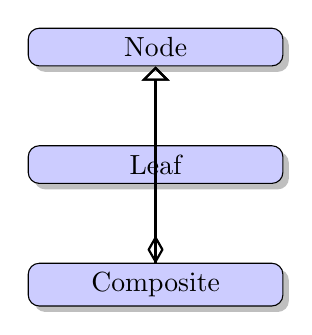
\begin{tikzpicture}[node distance=1cm,>=stealth',bend angle=45,auto]
    \tikzstyle{class}=[rectangle, draw=black, rounded corners, fill=blue!20, drop shadow,
        text centered, anchor=north, text=black, text width=3cm]
    \tikzstyle{interface}=[rectangle, draw=black, rounded corners, fill=red!20, drop shadow,
        text centered, anchor=north, text=black, text width=3cm]
    \tikzstyle{inheritance}=[->, >=open triangle 90, thick]
    \tikzstyle{realization}=[->, >=open triangle 90, thick]
    \tikzstyle{dependency}=[->, >=open triangle 90, thick]
    \tikzstyle{association}=[->, >=open triangle 90, thick]
    \tikzstyle{aggregation}=[->, >=open diamond, thick]
    \tikzstyle{composition}=[->, >=open diamond, thick]

    \node [class] (Node) {Node};
    \node [class, below=of Node] (Leaf) {Leaf};
    \node [class, below=of Leaf] (Composite) {Composite};

    \draw[inheritance] (Leaf) -- (Node);
    \draw[inheritance] (Composite) -- (Node);
    \draw[aggregation] (Composite.north) -- ++(0,0.5) -| (Composite.north);

\end{tikzpicture}
\caption{Class diagram}
\end{figure}

\end{document}
